\documentclass[12pt, a4paper, oneside, titlepage]{book}%[a4paper, final]{report}{article}
%%#################### PACKAGES DE BASE ####################################
\usepackage[french,frenchb]{babel} %%adapte les règles typographique en fonction de la langue - sans option, choisit la langue en fonction de celle définie dans la classe du document
\usepackage[T1]{fontenc} %-
\usepackage[utf8]{inputenc}%-[latin1]{inputenc}
%%#################### MISE EN PAGE #########################################
\usepackage[fs]{umons-coverpage}
\usepackage{fancyhdr} % Required for custom headers
\usepackage{graphicx} % pour afficher, redimensionner des images
\usepackage{lastpage} % pour pouvoir numéroter les pages << page xx sur 'lastpage'>>
\usepackage{caption} %pour mettre les images dans la marge
\usepackage{hyperref} % pour utiliser les liens hypertextes
\usepackage{xcolor} % pour colorer le texte
%\usepackage{extramarks} % Required for headers and footers
%\usepackage{pifont} % pour les puces personnalisées/caractère spéciaux,...
%\usepackage{enumitem} % pour d'autres puces
%\usepackage{listings} % pour afficher du Code source
%\usepackage[backend=biber]{biblatex} % pour la bibliographie
%\addbibresource{biblio.bib} % pour la bibliographie
%%#################### MATHS #########################################################
%\usepackage{amsfonts}
%\usepackage{amssymb}
%\usepackage{amsthm}
%\usepackage{algorithmic}% pour include du pseudo code
\usepackage{amsmath}
\usepackage{algorithm}% pour include du pseudo code
\usepackage[noend]{algpseudocode}% pour include du pseudo code
\makeatletter
\def\BState{\State\hskip-\ALG@thistlm}
\makeatother

%%#################### TABLEAUX #######################################################
\usepackage{array}                       %est entre autre nécessaire pour centrer un tableau
%%#################### DIVERS (graphique, url, annexe, .eps, code) ####################
%\usepackage{tikz} % arbres
%\usetikzlibrary{arrows} pour définir des flèche dans les arbres
%\usepackage{times}
%\usepackage{rotate}
%\usepackage{lscape}
%\usepackage{verbatim}
%\usepackage{eurosym} % pour le symbole €
%\usepackage{caption} % pour la position des images
%\usepackage{float,caption} % pour la position des images
%\usepackage{cite} %permet d'ordonner plusieurs références citées en même temps et de les afficher sous la forme d'un intervalle si elle se suivent

\graphicspath{{Images/}} %pour l'emplacement des images
\newcommand{\labelfigure}[1]{figure~\ref{#1} (page~\pageref{#1})}
\newcommand{\annexe}[1]{annexe~\ref{#1} (page~\pageref{#1})}
%\newcommand{\smalltitle}[1]{\bigskip\large\textbf{#1}\par\normalsize\medskip}



%%#################### START CHANGE HERE ###################################
\author{Sophie Opsommer}
\title{Mémoire : }
\umonsAuthor{\begin{tabular}{lll}
\textsc{Opsommer} & Sophie & SOPHIE.OPSOMMER@student.umons.ac.be\\
\end{tabular} }
%% The main title of your thesis
\umonsTitle{Mémoire : Database Repairing with Respect to Functional Dependencies }
%% The sub-title of your thesis
\umonsSubtitle{Mémoire réalisé dans le cadre \\du Master en Sciences Informatiques, à finalité spécialisée}
%Service : Neurosciences, Facult´e de M´edecine et de Pharmacie
%% Your supervisor(s)
\umonsSupervisor{\begin{tabular}{ll}
\textit{Directeur} : & J. \textsc{Wijsen} \\
%%\textit{Rapporteur} : & T. Mens\textsc{} \\
\end{tabular}}
%% The date (or academic year)
\umonsDate {2018-2019}
%%#################### END CHANGEMENT ##################################

%%#################### SET UP THE HEADER AND FOOTER ####################
\fancyhf{}
\chead{\leftmark}
%\rhead{\firstxmark} % Top right header
%\cfoot{} % Bottom center footer
\rfoot{Page \thepage\ sur \protect\pageref{LastPage}} % Bottom right footer
\setlength{\headheight}{15pt}

\begin{document}
%%#################### Page de présentation (pour le secrétariat) 
%###################### feuille volante à fournir en plus du mémoire :
\thispagestyle{empty}
\begin{center}

\includegraphics[height=2cm]{UMONS-Logo.jpg}\\
\textnormal{\Large{Faculté des Sciences}}\\
\textnormal{\Large{Département d'Informatique}}
\end{center}

\vspace*{2cm}
\begin{center}
\fbox{
\begin{minipage}{15cm}
\center
\vspace*{0.5cm}
\textbf{\LARGE{Mémoire : }}\\[0.5em]
\textbf{\LARGE{Database Repairing with Respect to Functional Dependencies}}\\\vspace*{0.5cm}
\end{minipage}
}
\end{center}

\vspace*{2cm}
\large{
\begin{center}
\begin{tabular*}{14cm}{@{\extracolsep{\fill}}lr}
Directeurs : M\textsuperscript{r} Jef \textsc{Wijsen} & Projet réalisé par\\
 & Sophie \textsc{Opsommer}\\[1em]
Rapporteur :  & \\
\end{tabular*}
\end{center}}

\vspace*{4cm}
\begin{center}
Année académique 2018-2019
\end{center}
\pagebreak

\newpage
\frontmatter % numérotation en chiffres romains

%%#################### Page de couverture ####################(cf fichier umonscoverpage.sty)
\thispagestyle{empty}
\umonsCoverPage
\pagebreak

\newpage
\thispagestyle{empty}
\pagenumbering{roman}  %\pagenumbering{gobble}
\vspace*{\stretch{1}}
\chapter*{}
%\begin{abstract}
Ce \emph{rapport de projet} est rendu dans le cadre du cursus de \og Master en sciences informatiques, à finalité spécialisée \fg. Le but de ce rapport est de présenter le problème qui est posé, de développer l'analyse du problème et les choix réalisés ainsi que d'exposer la réalisation.
%\end{abstract}
\vspace*{\stretch{1}}

\cleardoublepage
\newpage
%%#################### Acknoledge ####################
%//Remerciements (facultatif) bon example dans le livre de référence musimoti
\thispagestyle{empty}
\vspace*{\stretch{1}}
REMERCIEMENTS
%Dès à présent, je voudrais remercier tous ceux qui m'ont aidé dans ce projet. Certains sont des professeurs, des experts ou alors des amis avec lesquels j'ai eu l'occasion de partager des discussions sur des points techniques ou pratiques. D'autres sont des membres de ma famille qui m'ont soutenu, montré de l'intér\^et pour le projet et/ou relu mes écrits, ...

%Je pense en particulier au Professeur L. Ris du département de \emph{Médecine} de l'université qui a proposé ce sujet, m'a aidé à rédiger le cahier des charges en prenant le temps de m'expliquer point par point ce qu'elle souhaitait et qui à pris le temps à plusieurs reprises de tester les délivrables présentés et de me fournir des comptes-rendus constructifs et détaillés. Merci également au Professeur B. Quoitin pour son temps, sa patience et ses conseils tout au long du projet, à Benoit Debled, Danny Willems, Valentin Lecomte, Lucas Vanoverberghe, Jérémie Vincke et Dorian Opsommer pour les informations fournies, leur point de vue et leurs connaissances techniques et enfin, je tiens à remercier toutes les personnes qui m'ont conseillé et relu lors de la rédaction de ce rapport de projet.

%Sans oublier Mr V. Boulanger du \emph{service informatique de l'UMONS} pour ses réponses, sa disponibilité et la mise à disposition du serveur ainsi que Dr S. Brognaux du service \emph{Administration et Valorisation de la Recherche (AVRE) de l'UMONS} pour son aide à déposer le projet sur les stores d'applications mobiles.
% + Mr quoitin pour son Mac

\vspace*{\stretch{1}}
%%#################### TABLE OF CONTENTS ####################
\newpage
\thispagestyle{empty}
\tableofcontents
%N.B. : avec tocbibind il y aurait moyen d'ajouter les tableau dans la table des matières.
      
%%#################### LE RAPPORT COMMENCE ICI ####################
\newpage
\pagestyle{fancy}  % headings (nom du chapitre et le numéro de page en en-t\^ete), plain(numéro de page au milieu du pied de page), empty
\mainmatter  % start of the contributions chapitre numéroté en chiffres
\chapter{Introduction}\label{CHintro}
...
\vspace*{20mm}
%Brève description du contenu chapitre par chapitre
%Dans la suite de ce rapport seront présentés ... Enfin la conclusion contient le mot de la fin avec les améliorations possible et un avis personnel rétro-actif. 

%Dans les annexes se trouvent la bibliographie, un glossaire des termes techniques utilisés et des suppléments informations pouvant étayer certaines parties du rapport.

\cleardoublepage % permet de recommencer à écrire sur la page impaire (belle page) % bibitem : https://fr.wikibooks.org/wiki/LaTeX/Faire_des_tableaux
%%%%%%%%%%%%%%%%%%%%%%%%%%%%%%%%%%%%%%%%%%%%%%%%
%%%%%%%%%%%%%%%%%%%%%%%%%%%%%%%%%%%%%%%%%%%%%%%%
\chapter{Contexte}\label{CHcontexte}
(deviendra peut-être l'introduction)

\`{A} l'heure où le monde collecte et enregistre de plus en plus de données et qu'il tente d'en tirer des conclusions et des prédictions, vérifier l'exactitude des informations devient aussi de plus en plus importante. Il existe beaucoup de critères à vérifier et beaucoup de méhodes pour y arriver.

Interessons-nous à l'un d'entre eux : les dépendances fonctionelles.

Dans la pratique, il peut arriver que des dépendances ne sont pas respectées. Les causes sont multiples :
\begin{itemize}
\item Une manipulation volontaire (pour une situation d'exception), 
\item Une erreur manuelle d'encodage ou de manipulation involontaire, 
\item Une source de données imprécise (par le biais d'internet, de capteurs avec des marges d'erreurs,...), 
\item Une méthode de collecte imprécise (reconnaissance vocale, analyse de signaux, d'image,...)
\item Un rappatriement de données provenant de plusieurs sources avec des données différente ou avec des formats différents,
\item Une mauvaise vérification au niveau applicatif,
\item L'utilisation de plusieurs applications qui ne respectent pas toutes les mêmes règles et procédures,
\item ...
\end{itemize}

Il est important de corriger la situation (et de trouver la méthode optimale pour y arriver) parce que la qualités des informations joue un rôle important dans la qualités du traitement des données ultérieurement. Comme le dit le jargon/proverbe : \og shit in, shit out \fg. Ce qui revient à exprimer que si les données avec lesquelles on travaille ne sont pas credible, les conclusions que l'on pourra en tirer ne le seront pas non plus. En cas d'audit, ça permet aussi de calculer le degré ?d'inconsistence? de la table (on calculera la distance entre la base de données initiale et corrigée). 

Pour remédier à ces erreurs, il faut d'une part remédier à la cause de ces incohérences mais aussi corriger les données qui sont incorrecte ou qui ont été corrompue. Pour la correction, il y a 2 solutions. Soit modifier les requêtes pour que celles-ci ne renvoient que les lignes non concernées par ces incohérences. Soit il faut trouver une base de données à l’image de la base de données existante qui, après un minimum de changements, respecte les contraintes d’intégrités. Pour cette dernière solution, deux possibllités existent également. On peut supprimer les données qui sont incorrecte ou on peut modifier les données incorrectes.

Dans la suite, nous traiterons d'une méthode possible pour corriger les données existantes par le biais de la suppression des données incohérentes avec les dépendances fonctionnelles.



\clearpage
%%%%%%%%%%%%%%%%%%%%%%%%%%%%%%%%%%%%%%%%%%%%%%%%
%%%%%%%%%%%%%%%%%%%%%%%%%%%%%%%%%%%%%%%%%%%%%%%%

\section{Notions de bases}\label{SECbase}
Avant de rentrer dans le vif du sujet, voici un bref rappel de certaines notions de base. Toute personne habituée à travailler dans le domaine des bases de données peut alègrement sauter cette section et passer à la suivante.


\subsection{Une contrainte d'intégrité : } 
Les contraintes d'intégrités sont les assertions qui doivent être vérifiées par les données contenues dans la base de données. Elles regroupe différentes catégories comme : 
\begin{description}
\item {les intégrités de domaine :} les valeurs d'un attribut doivent appartenir au domaine de valeurs de l'attribut.
\item {les intégrités de clé :} les clés d'une tables sont uniques et non nulle.
\item {les intégrités référentielle :} les clés étrangères sont nulles ou référence une clé primaine existante.
\end{description}

\subsection{Une dépendance fonctionnelle : }
Une dépendance fonctioenlle est une contrainte sémantique. Elle est supposée toujours vrai dans le monde réel.

C'est une relation entre plusieurs attributs d'une même table. Elle definit la valeur d'un attribut (ou d'un ensemble d'attributs) en fonction d'un autre ou de plusieurs autres attributs. En effet la dépendance fonctioennelle $ X \rightarrow Y$ définit que si plusieurs lignes ont les mêmes valeurs pour un ensemble $X$ d'attributs, elles auront également les mêmes valeurs pour l'ensemble $Y$ d'attributs.
En terme de notation, on dira : soit la table de référence T définit par la relation $R{a_1, a_2, a_3,...,a_n}$ avec n le nombre d'attribut et X et Y des sous-ensemble de R. On dit que \og Y dépend fonctionnellement de X \fg ou \og X détermine Y \fg 0si à chaque valeur de X correspond une valeur unique de Y. On écrit alors \og $ X \rightarrow Y$ \fg.

\begin{figure}[ht]
	\center
	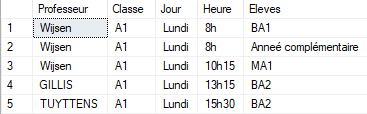
\includegraphics{DF.png}
	\caption{\label{picDF} Extrait d'une table pour illustrer des dépendances fonctionnelles}
\end{figure}

Par exemble, la table illustrée dans la figure \ref{picDF} pourrait exister dans une école. Elle illustre les différents professeurs, la classe (emplacement physique) où ils enseignent à un jour et une plage horraire précise ainsi que les élèves qui seront présent. Avec les lois spacio-temporrelle que nous connaissons, un professeur ne peut se trouver que dans une classe à la fois. En terme de dépendance, cela signifie qu'à un jour de la semaine, une plage horaire et un professeur ne peut donc correspondre qu'une seule classe. Notons par contre que des élèves d'années différentes peuvent y assister en même temps. Inversément, une classe n'est utilisée que par un professeur à la fois. De la même façon, des élèves ne peuvent se trouver que dans une seule classe à la fois
Ces dépendances s'écrivent : $\{Eleves, Jour, Heure \rightarrow Classe\}, \{Professeur, Jour, Heure \rightarrow Classe\}, \{Classe, Jour, Heure \rightarrow Professeur\}$.

\subsubsection{Une dépendance fonctionnelle élémentaire}
Une dépendance fonctionnelle élémentairetel $X \rightarrow A$ est un dépendance fonctionnelle où A est un attribut unique non inclus dans X et où il n’existe pas d'ensemble d'attribut X’ inclus dans X tel que $X’ \rightarrow A$.

\subsubsection{Une clé (primaire)}
Une clé est un attribut (ou un groupe minimum d'attributs) qui définit tous les autres attributs de la relation.

\subsection{Une opération}
Une opération est une manipulation qui est efectuée sur un ensemble de données pour obtenir un ou plusieurs nouvel ensemble de données.

\subsubsection{L'union}
L'union de deux relations R1 et R2 de même schéma est une relation R3 de schéma identique qui a pour n-uplets les n-uplets de R1 et de R2.
On notera : $R3 = R1 \bigcup R2$

\subsubsection{L'intersection}
L’intersection entre deux relations R1 et R2 de même schéma est une relation R3 de schéma identique ayant pour n-uplets les m-uplets communs à R1 et R2.
On notera : $R3 = R1 \bigcap R2$

\subsubsection{La différence}
La différence entre deux relations R1 et R2 de même schéma est une relation R3 de schéma identique ayant pour n-uplets les n-uplets de R1 n'appartenant pas à R2.
On notera : $R3 = R1 -  R2$

\subsubsection{La projection}
La projection d'une relation R1 est la relation R2 obtenue en supprimant les attributs de R1 non mentionnés puis en éliminant éventuellement les n-uplets identiques.
On notera : $R2 = \pi R1 (A_i, A_j, ... , A_m)$ la projection d'une relation R1 sur les attributs $A_i, A_j, ... , A_m$.
Î
 La projection permet d’éliminer des attributs d’une relation.  Elle correspond à un découpage vertical.

\subsubsection{La restriction}
La restriction d'une relation R1 est une relation R2 de même schéma n'ayant que les n-tuplets de R1 répondant à la condition énoncée.
On notera : $R3 = \sigma R1 (condition)$ la restriction d'une relation R1 suivant le critaire "condition" où "condition" est une relation d'égalité ou d'inégalité entre 2 attributs ou entre un attribut et une valeur.
La restriction permet d'extraire les n-tuplets qui satisfont une condition. Elle correspond à un découpage horizontal.

\subsubsection{La jointure}
La jointure de deux relations R1 et R2 est une relation R3 dont les n-uplets sont obtenus en concaténant les n-uplets de R1 avec ceux de R2 et en ne gardant que ceux qui vérifient la condition de liaison.
On notera : $R3 = R1 \ast  R2 (condition)$ la jointure de R1 avec R2 suivant le critère "condition". Le schéma de la relation résultat de la jointure est la concaténation des schémas des opérandes. S'il y a des attributs de même nom qui ne font pas partie de la condition, il faut les renommer. Si ils font partie de la condition, il seront fusionné ne n'apparaîtront qu'une seule fois. Les n-uplets de $R1 \ast R2 (condition)$ sont tous les couples (u1,u2) d'un n-uplet de R1 avec un n-uplet de R2 qui satisfont "condition". La jointure de deux relations R1 et R2 est le produit cartésien des deux relations suivi d'une restriction. La condition de liaison doit être du type : <attribut1>  ::  <attribut2> où :  attribut1 $\in$ 1ère relation, attribut2 $\in$ 2ème relation et :: est un opérateur de comparaison (égalité ou inégalité). La jointure permet de composer 2 relations à l'aide d'un critère de liaison.

%Jointure naturelle : Jointure où l'opérateur de comparaison est l'égalité dans le résultat on fusionne les 2 colonnes dont les valeurs sont égales. La jointure permet d'enrichir une relation
% La normalisation conduit à décomposer ; la jointure permet de recomposer.
%Auto-jointure : jointure d'une relation par elle-même

\subsubsection{La division}
Soit deux relations $R1 (A_1, A_2, ... , A_n, B_1, B_2, ... , B_m)$ et $R2 (B_1, B_2, ... , B_m)$.
Si le schéma de R2 est un sous-schéma de R1. La division de R1 par R2 est une relation R3 dont :
\begin{enumarate}
-  le schéma est le sous-schéma complémentaire de R2 par rapport à R1
-  un n-uplet (a1 , a2, ... , an) appartient à R3 si (a1, a2, ... , an, b1, b2, ... , bm) appartient à R1 pour tous (b1, b2, ... , bm) $\in$ R2.
\end{enumarate}
On notera : $R3 = R1 \div  R2$ la division de R1 par R2. La division permet de rechercher dans une relation les sous n-uplets qui sont complétés par tous ceux d'une autre relation. Elle permet de répondre à des questions qui sont formulées avec le quantificateur universel : "pour tout ...".

\subsection{La fermeture transitive}
La fermeture transitive permet d'enrichir une relation à 2 attributs de même domaine, avec tous les couples qui se déduisent par transitivité.

Soit par exemple, 2 attributs A et B qui ont pour domaine les chiffres.
Soit une table définie par la relation R(A,B) qui contient les données (1, 2) et (2, 3). La fermeture de cet ensemble est composée de (1, 2) et (2, 3) et (1, 3).
!! le domaine, c'est les chiffres ? ou c'est A = 1 et 2 et B = 2 et 3 ?????

%%%%%%%%%%%%%%%%%%%%%%%%%%%%%%%%%%%%%%%%%ù
\clearpage
%%%%%%%%%%%%%%%%%%%%%%%%%%%%%%%%%%%%%%%%%%%%%%%%
%%%%%%%%%%%%%%%%%%%%%%%%%%%%%%%%%%%%%%%%%%%%%%%%

\section{Notions complémentaires}\label{SECcomplement}
Ici seront détaillés des notions propre à ce travail qui ne seront peut-être pas commun aux standarts de notations habituels. Il est donc important de les comprendre avant de poursuivre la suite de la lecture.

!! commencer par définir les notations comme delta !!

\subsection{Un attribut commun à la main gauche : } 
est un attribut « A » qui se trouve dans toutes les parties gauches des dépendances fonctionnelles de $\Delta$. Dans l'exemple de la figure \ref{picDFs}, l'attribut \fg Facility \og est donc un attribut commun à la main gauche. En présence de ce type d'attribut, trouver les données de la table initiale qui composeront la solution optimale reviendra à traité independamment les lignes en les groupant par la valeur de cet attribut et ensuite en faisant l'union des sous-ensembles.  De cette manière, pour chaque sous-ensemble, cet attribut n'a qu'une seule valeur et peut donc être supprimé dans les dépendances fonctionnelles.

Dans l'exemple de la figure \ref{picDFnok} cela reviendrait a traiter d'une part les 3 premières lignes et d'autre part la dernière. Les dépendances deviennent donc : $\{ \emptyset \rightarrow City \} et \{  Room \rightarrow Floor \}$.

\subsection{Un consensus : } 
est une dépendance fonctionnelle dont la main gauche est vide : $\emptyset \rightarrow Y$. Cette dépendance fonctionnelle est respectée si la valeur du ou des attributs de Y est toujours identique. En présence de ce type d'attribut, trouver les données de la table initiale qui composeront la solution optimale reviendra à grouper les lignes avec la même valeur pour le ou les attributs $Y$ de la main droite de la dépendances. Ensuite plutôt que de faire l'union des sous-ensembles comme précédement, il conviendra de choisir l'un des sous-ensemble. Pour faire ce choix, il faut calculer la distance que la suppression de chacun des groupes impliquerait et prendre le groupe de ligne avec la distance la plus faible. Ensuite, la main droite de la dépendance étant identique pour toutes les lignes du sous-ensemble, cette dépendance peut être supprimée.

Dans l'exemple de la figure \ref{picDFnok}, après avoir traité l'attribut commun, nous avons la dernière ligne qui respecte les contraintes et les trois autes pour qui il y a encore du travail. Traiter le consensus reviendrait à garder la première ligne ou les lignes 2 et 3. Si on garde la première ligne (et donc qu'on supprime les deux autres), la distance entre la table T initiale et la table image T' est $dist_{sub}(T, T') = 1+ 1 = 2$ or si ongarde les deux autres, la distance est de $dist_{sub}(T, T') = 3$. Garder la première ligne est donc la meilleure solution. Maintenant, $\Delta = \{  Room \rightarrow Floor \}$. Et notre sous-ensemble respecte cette dépendance donc le tour est joué.

\subsection{Une chaîne : } 
est une dépendance fonctionnelle qui en inclus une autre.
....

\subsection{ Un mariage : }
est une situation où la table présente plusieurs identifiants. Chacun d'eux va alors déterminer le ou les autres identifiants. Par exemple $\Delta = \{  X \rightarrow Y \}, \{  Y \rightarrow X \}$. On dit que leur ""closure"" sont identiques. et il faut également que l'un deux soit présent dans chacune des autres dépendances, par exemple $\Delta = \{  X \rightarrow Y \}, \{  Y \rightarrow X \}, \{ X \rightarrow Z\}$.
+ complément video 0:8:00



\clearpage
%%%%%%%%%%%%%%%%%%%%%%%%%%%%%%%%%%%%%%%%%%%%%%%%
%%%%%%%%%%%%%%%%%%%%%%%%%%%%%%%%%%%%%%%%%%%%%%%%

\section{Notations}\label{SECnotations}
Pour pouvoir transcrire le problème en notation mathématique, voici les raccourcis utilisés : 
\begin{description}
\item{$D$ : } la base de données source incohérente % elle peut être relationnelle, hierarchique, en réseau,... puisqu'on ne travaille que sur 1 table.
\item{$D'$ : } image de D qui soit cohérente
\item{$T$ : } table unique de la base de données D. Chaque ligne est numérotée par un identifiant qui ne sera jamais modifié. Il permet d'avoir un lien entre la version D et D' de la base. Elles sont aussi caractérisée par un poid qui détermine combien coûte la suppression de cette ligne. La table peut-être avec ou sans doublons et pondérée ou non. Si elle n'est pas pondérée, on fixera le même poids à toutes les lignes.
\item{$T'$ : } image de T qui soit cohérente
\item{$R$ ou $R(a_{1}, ... , a_{k})$ : } schéma relationnel de la table T où chaque $a_i$ est un attribut. Cette relation est un sous-ensemble du produit cartésien de plusieurs domaines de valeurs.
\item{$Val$ : } domaine (infini?) de valeur d'attribut
\item{$T[i]$ : } la ligne i de la table T
\item{$T[*]$ : } toutes les lignes de T
\item{$ids(T)$ : } identifiant de la ligne i de la table T ???
\item{$Val^k$ : } domaine de valeur de l'attribut k. Il s'agit de l'ensemble des valeurs que l'attribut est succeptible de prendre.
\item{$w_T(i)$ : } poids de la ligne i de la table T
\item{$|T| = |ids(T)|$ : } le nombre de ligne de T
\item{$t = (a_1, ..., a_k$ : } est une ligne de la table T
\item{$t.A_j$ : } référence vers la valeur de $a_j$
\item{$A, B,C,..., X, Y, Z$ : } Les premières lettres de l'alphabet illustrent un seulattribut à la fois alors que les dernières lettres de l'alphabet représententun ensemble d'attribut.
\item{$\Delta$ : } ensemble des dépendances fonctionelles
\item{$X \rightarrow Y$ : } expression d'une dépendance fonctionnelle où X et Y sont des séquences d'attribut
\item{$lhs ou rhs$ : } \fg left/right hand side \og, on évoque la partie gauche/droite de la dépendance fonctionnelle.
\item{$\Delta |= X \rightarrow Y$ : } la dépendance fonctionnelle est ?implique? dans $\Delta$. C'est-à-dire que si une table vérifie $\Delta$, elle vérifie aussi $X \rightarrow Y$.
\item{$Cl(\Delta)$ : } la fermeture de delta. Elle regroupe la liste exhaustive detoutes les dépendances fonctionnelle qui sont ?impliquée? par delta.
\item{$Cl_\Delta(X)$ : }  la fermeture d’un attribut (ou d’une séquence d‘attribut) X. C’est la liste de tous les attributs A tel que $X \rightarrow A$ est impliquée dans $\Delta$.
\item{$\Delta1 = \Delta2$ : } si leurs fermetures sont identique.



\item{ : } 
\item{ : } 
\item{ : } 
\item{ : } 
\item{ : } 
\item{ : } 
\item{ : } 
\item{ : } 
\item{ : } 
\end{description}
...
\clearpage
%%%%%%%%%%%%%%%%%%%%%%%%%%%%%%%%%%%%%%%%%%%%%%%%
%%%%%%%%%%%%%%%%%%%%%%%%%%%%%%%%%%%%%%%%%%%%%%%%
\chapter{Sous-ensemble optimal}\label{CHsrepair}
Pour obtenir une version de la base de données cohérente avec un minimum de suppression de ligne, l'article \cite{article} expose une solution. Les auteurs proposent un algorithme qui, sur base des dépendances fonctionnelles, prédit un problème polynomial ou APX-complet (sous-ensemble de la classe NP-difficile). Si le probème est de complexité polynomiale, alors une solution en un temps polynomial peut être trouver et ce, même si la table est lourde et/ou comporte des doublons. Dans le cas contraire, le problème ne peut qu'être approximé à une constante prêt.

La méthode de correction évaluée tiendra compte du caractère optimal de la solution. Pour se faire elle calculera la distance entre la la base de donnée source et son image. Cette distance sera calculée en additionnant le poid des lignes supprimées.
Dans l'exemple de la figure \ref{picDFnok}, supprimer la première ligne, sera plus coûteux que de supprimer les deux suivantes. Pour respecter les dépendances fonctionnelles suivante : $\{ Facility \rightarrow City \} et \{ Facility, Room \rightarrow Floor \}$, on supprimera donc les lignes 2 et 3 pour obtenir le sous-ensemble optimal.

\begin{figure}[ht]
	\center
	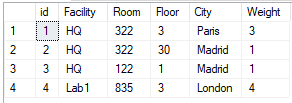
\includegraphics{DFnok.png}
	\caption{\label{picDFnok} Extrait d'une table pour illustrer des dépendances fonctionnelles particulières}
\end{figure}


\section{OSRSucceeds($\delta$)}

Cet algorithme a été écrit pour prédire la complexité de la correction. Il va en effet travailler uniquement sur les dépendances fonctionnelles en ne tenant pas compte des données. Si l'algorithme est un succès, cela signifie qu'il aura réussi à simplifié les dépendances et à les substituée pour ne plus les traiter que une par une. Il est alors possible de lancer l'algorithme de correction des données qui mettra un temps polynomial à s'exécuter. Par contre si l'algorithme est un échec, alors il ne sera pas possible de corriger les données avec l'algorithme proposé dans un temps polynomial.

Voici le pseudo code de ce premier algorithme : 
\begin{algorithm}
\caption{OSRSucceeds}\label{euclid}
\begin{algorithmic}[1]

\BState $\emph{while} \Delta is nontrivial \emph{do} :$
\State $remove trivial FDs from \Delta$
\If $\Delta has a common lhs A then$
\State $\Delta := \Delta - A$
else if $\Delta has a consensus FD \emptyset \rightarrow A then$
\State $\Delta := \Delta - A$
else if $\Delta has an lhs marriage (X1,X2) then$
\State $\Delta := \Delta - X1X2$
else
\State $\textbf{return} false$
\EndIf
\State $\textbf{return} true$

\end{algorithmic}
\end{algorithm}

\begin{algorithm}
\caption{OSRSucceeds}\label{euclid}
\begin{algorithmic}[1]
\Procedure{Simplify}{$\Delta$}
\State $\textit{stringlen} \gets \text{length of }\textit{string}$
\State $i \gets \textit{patlen}$
\BState \emph{top}:
\If {$i > \textit{stringlen}$} \Return false
\EndIf
\State $j \gets \textit{patlen}$
\BState \emph{loop}:
\If {$\textit{string}(i) = \textit{path}(j)$}
\State $j \gets j-1$.
\State $i \gets i-1$.
\State \textbf{goto} \emph{loop}.
\State \textbf{close};
\EndIf
\State $i \gets i+\max(\textit{delta}_1(\textit{string}(i)),\textit{delta}_2(j))$.
\State \textbf{goto} \emph{top}.
\EndProcedure
\end{algorithmic}
\end{algorithm}


\clearpage
%%%%%%%%%%%%%%%%%%%%%%%%%%%%%%%%%%%%%%%%%%%%%%%%%
%%%%%%%%%%%%%%%%%%%%%%%%%%%%%%%%%%%%%%%%%%%%%%%%%
\section{OptSRepair($\Delta, T$)}
...
$
1: if \Delta is trivial then \% successful termination
2: return T
3: remove trivial FDs from \Delta
4: if \Delta has a common lhs then
5: return CommonLHSRep(\Delta,T )
6: if \Delta has a consensus FD then
7: return ConsensusRep(\Delta,T )
8: if \Delta has an lhs marriage then
9: return MarriageRep(\Delta,T )
10: fail \% cannot find an optimal S-repair
$

\section{CommonLHSRep($\Delta, T$)}
...
$
1: A := a common lhs of \Delta
2: return \cup_{(a)\in \pi_{A}T[*]}OptSRepair(\sigma_{A=a}T, \Delta - A)
$

\section{ConsensusRep($\Delta, T$)}
...
$
1: select a consensus FD \emptyset \rightarrow  A in \Delta
2: for all a \in \pi_A T [*] do
3: S_a := OptSRepair(\sigma_{A=a}T, \Delta - A)
4: a_{max} := argmax_a \{w_T (S_a ) | (a) \in  \sigma_A T [*]\}
5: return S_{a_{max}}
$

\section{MarriageRep($\Delta$, T)}
...
$
1: select an lhs marriage (X_1, X_2) of \Delta
2: for all (a_1, a_2) \in  \pi{X_1 X_2} T [*] do
3: S_{a_1, a_2} := OptSRepair(\sigma_{X_1 = a_1, X_2 = a_2}T, \Delta - X_1 X_2)
4: w(a_1, a_2) := w_T (S_{a_1,a_2} )
5: V_i := \pi_{X_i}T [*] for i = 1, 2
6: E := \{(a_1, a_2) | (a_1, a_2) \in  \pi_{X_1 X_2}T [*]\}
7: G := weighted bipartite graph (V_1,V_2, E,w)
8: E_{max} := a maximum matching of G
9: return \cup_{(a_1, a_2 )\in E_{max}}S_{a_1, a_2}
$











\clearpage
%%%%%%%%%%%%%%%%%%%%%%%%%%%%%%%%%%%%%%%%%%%%%%%%%%%%%%%
%%%%%%%%%%%%%%%%%%%%%%%%%%%%%%%%%%%%%%%%%%%%%%%%%%%%%%%
\appendix
\bibliographystyle{plain}
\begin{thebibliography}{9}
\bibitem {video} \url{https://www.youtube.com/watch?v=dXoLmFDbq7E}, 30/11/2018.
\bibitem {article} \textsc{Ester Livshits, Benny Kimelfeld, Sudeepa Roy}, \textit{ “Computing Optimal Repairs for Functional Dependencies”}, PODS. ACM, 2018, pp. 225–237.
\bibitem {BDD1} \textsc{Josef Wijsen}, {Syllabus}
\bibitem {coursNice} \url{https://www.i3s.unice.fr/~nlt/cours/licence/sgbd1/sgbd1_cours.pdf}, 15/12/2018.
\end{thebibliography}

%replace : 
%î 		\^{i}
% ê		\^{e}
% ù 		\`{u}
% è		\`{e}
% à		\`{a}
% é		\'{e}
% ç		\c{c}
%delta	$\Delta$
\end{document}





